\chapter{Background and Research}
This chapter will look at explaining the neccessary requirements to understanding the project. It will explain the functionality and applications of cryptographic hashing algorithms, before looking deeper into SHA-3, explaining the algorithms' origin and how it works. Finally, it will review similar work published by different authors and the software that has been developed alongside of it.
\section{Cryptographic Hashing Algorithms Overview}
\subsection{Brief History}
The first of many cryptographic hash functions was created in the late 1970's but the topic did not gain any noticeable momentum until the early 90's when the first widely used algorithms became popularised. These algorithms are known as MD5 and SHA-1 and were the first cryptographic hashing algorithms to be included in a wide number of applications.
\vspace{5 mm}\\
Throughout the start of the new millennium, cryptographers found serious security flaws in both MD5 and SHA-1, forcing significant progress to be made in the field. SHA-2, which had already been created prior to these weaknesses being discovered, had many similarities to SHA-1 but the same weakness could not seem to be used to exploit the SHA-2 algorithm in the same way. \vspace{5 mm}\\
After the weaknesses in SHA-1 and MD5 became exposed, NIST (National Institute of Standards and Technology) announced a competition to create the next member of the SHA family, SHA-3. It was decided that the algorithm should be designed separately to SHA-1 and SHA-2 in case further weaknesses were yet to be exposed. In 2013, NIST began the standardisation process for the algorithm and in late 2014, they published a draft of SHA-3.\cite{SHA3comp}
\subsection{Functionality}
A cryptographic hash function has one primary goal, which is to be used as a map from some input string, the message, to an output string of a fixed length, the hash value. To ensure the hash function is secure, it is required that it is ``practically impossible" to invert in addition to having a very low probability of 2 input strings producing the same output string. In other words, given a hash value it would be ``hard" to discover what message generated such a value.  A more precise definition is used by cryptographers which will be examined more closely further into this thesis. Difficulty, such as uses of the word ``hard", can be quantified.
\subsection{Applications}
Cryptographic hash functions have a wide range of uses in computer science including password verification and pseudorandom generators.
\subsubsection{Password verification}
Clearly, storing all passwords in plain text is serious security risk, since if an adversary gains access to the database, they will immediately have access to all users' password. A widely used and trusted alternative to this is to use a process called ``hash and salt''.
\vspace{10mm}\\
HASH AND SALT PARAGRAPH HERE!!!!
\vspace{10mm}\\
 where as the password is created or changed you immediately apply a hash algorithm to the password and store this instead. Then when the user comes to log into their account the next time you can apply the same hashing algorithm to the entered password and compare this to the password stored in the file. This is still very insecure, so for added security a randomly generated string, called a salt, is concatenated to the password before the hashing algorithm is applied, then stored alongside the hash value for future references.
\vspace{10mm}\\
THINK ABOUT RE-WORDING ABOVE PARAGRAPH.
\vspace{10mm}\\
\subsubsection{Integrity of Data}
Checking to see if a message or file has been altered is an important process which must be completed. One way to achieve this is to calculate the hash value of the data. By taking the binary representation of the data, we can apply the hash algorithm to this string and return the hash value. Then when the message is sent to the recipient, the hash value is sent alongside it, both of which are encrypted. Upon receiving both, the recipient applies the same hash algorithm to the message and compares this with the hash value. If they match, the recipient can confirm with a high degree of certainty that the data has not been altered in transmission.

Clearly illistrate that the hash value is sent ALONGSIDE THE MESSAGE.

\subsubsection{Pseudorandom Generators}
Hash functions can be used to generate pseudorandom strings of a fixed length, which can be used as a private or public key for an encryption system. Giving the hashing algorithm different messages, or seeds as they are more commonly known, when the hash algorithm is being used as a pseudorandom generator, gives different unpredictable outputs. Each output can be considered to be a different random number.
\subsection{SHA-3}
SHA-3 is the hashing algorithm which will be looked at in much more detail in this project. Therefore a more in-depth explanation of what SHA-3 is will need to be given.
\vspace{5 mm}\\
SHA-3, like other hashing algorithms, takes an input and outputs an unpredictable, irreversible string of a fixed, predetermined length. It does this by taking the input string and padding this string to a required length. This string is then XORed into the state.

\begin{figure}[h]
\label{fig:stateFigure}
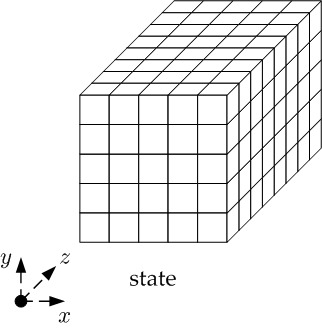
\includegraphics[width=5cm]{State}
\centering
\caption{SHA-3 State \cite{KeccakSite}}
\label{fig:stateFigure}
\end{figure}
\noindent The aforementioned state is a bit string represented in a specific format and is represented as a 3-dimensional array of size $5 \times 5 \times 64$, initialised completely to 0 at first. An illustrative example, although with smaller dimensions, of the state is given in figure~\ref{fig:stateFigure} \cite{KeccakSite}.\footnote{A state has size $ 5 \times 5 \times 64 $ if the `complete' SHA-3 algorithm is being used. Although for lighter weight applications, a smaller state may be used providing the size is of the form $5 \times 5 \times 2^{l}$ where $l$ is some integer less that $6$. Further information surrounding this is discussed in the appendix.}
\vspace{5 mm}\\
To absorb the input string into the state, we take the first $r$ bits of the string, where $r$ is predefined, and XOR these bits with the first $r$ bits of the state. Next, the block permutations are applied, transforming the current state into an alternative state. This will be explained in a greater detail in the following paragraph. If any bits remain in the input string, the process is repeated with the next $r$ bits until the string is completely absorbed, or alternatively until we are left with the empty string. This type of structure is known as a sponge construction.
\vspace{5 mm}\\
The block permutation is made up of 24 rounds, and each round is almost identical to every other. Rounds are made up of 5 sub-rounds which, when applied to the state, transforms it in some way.
\vspace{5 mm}\\
The first 4 sub-rounds, named $\theta$, $\rho$, $\pi$ and $\chi$, follow the same algorithm identically each time, whereas the final permutation, $\iota$, relies upon which round is currently being completed. When these 5 sub-rounds are performed one after the other, in the order given, the algorithm is said to have completed 1 round. For each block permutation to be completed, 24 rounds are completed in succession.
\vspace{5 mm}\\
\textit{Appendix A gives a more mathematical, in-depth explanation of SHA-3.}
\section{Previous Research}
After extensive research into the field of study, no discovery has been made of another piece of software which offers a solution to the problem which has been set out by this project. However, similar visualisation applications exists for both SHA-1 and SHA-2. One of the most popular papers produced, named SHAvisual: A Secure Hash Algorithm Visualization Tool \cite{SHAvisual}, created a visualisation tool for SHA-512 to aid both students and instructors in the learning and the teaching of the secure hashing algorithm. The algorithm demonstrated the major components of the algorithm in a step-by-step structure, whilst also providing a simplified version to be used in presentations. The tool also offers a `full mode' which can be used to perform full SHA-2 hashing. 
\vspace{5 mm}\\
Another paper\cite{VisSHA1} published focused more closely on SHA-1 and creating an applet which looks into the weaknesses and strengths of SHA-1, whilst also producing an ``interactive visualisation for teaching SHA-1". The paper, Visualizing Secure Hash Algorithm (SHA-1) on the Web, looks to gain knowledge about the algorithm, SHA-1, and then further looks to evolve the applet for use with SHA-2. This project looks to implement a similar application, to be embedded into the web for use with SHA-3.
